\section{Assignment 14}

\subsection{Implement the force control with inner position loop}

\begin{figure}[h]
\centering
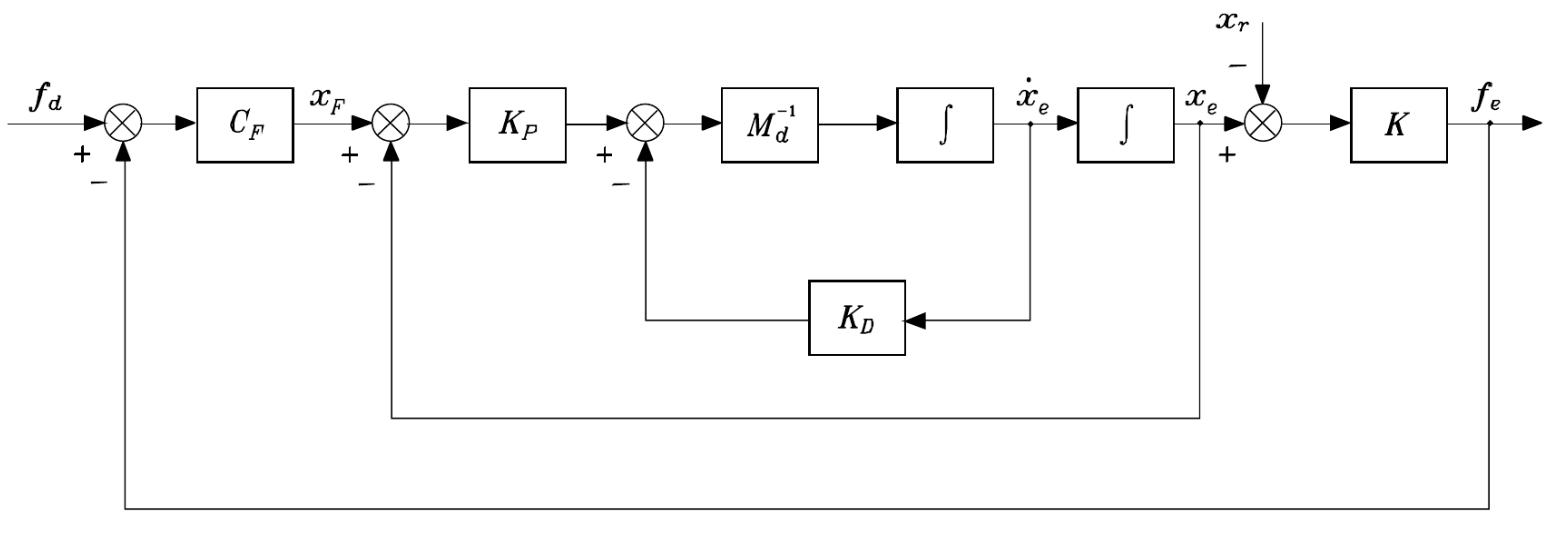
\includegraphics[keepaspectratio,width=0.8\textwidth]{force_arch}
\caption{Force control with inner position loop architecture.}
\end{figure}

The architecture is based on an inverse dynamic position control surrounded by a force feedback loop. Given a desired constant force reference $f_d$ we define a diagonal matrix $C_F$ that acts like a compliant matrix, mapping force into position:

\begin{equation*}
x_F = C_F(f_d-f_e)
\end{equation*}

where $f_e$ is the measured interaction force.

The shape of the controller $C_F$ is important. If $C_F$ is a PI controller, i.e. $C_F=K_F+\frac{1}{s}K_I$, then the steady state error is null.

The architecture is modelled in SIMULINK as follows:

\begin{figure}[h]
\centering
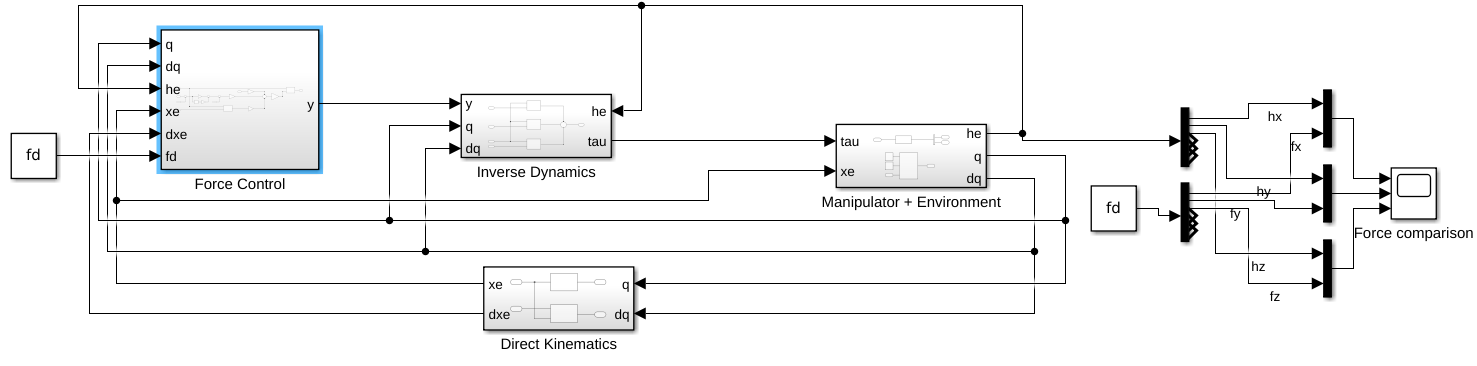
\includegraphics[keepaspectratio,width=0.8\textwidth]{force_sim}
\caption{Force control with inner position loop SIMULINK model.}
\end{figure}

The architecture was tested with $f_d = \begin{bmatrix}
0 & 1 & 0 & 0 & 0 & 0
\end{bmatrix}$, with an environment stiffness $K=5\mathbb I_6$, PI gains for the force loop $K_I=5\mathbb I_6$ and $K_F=10\mathbb I_6$.

\begin{figure}[h]
\centering
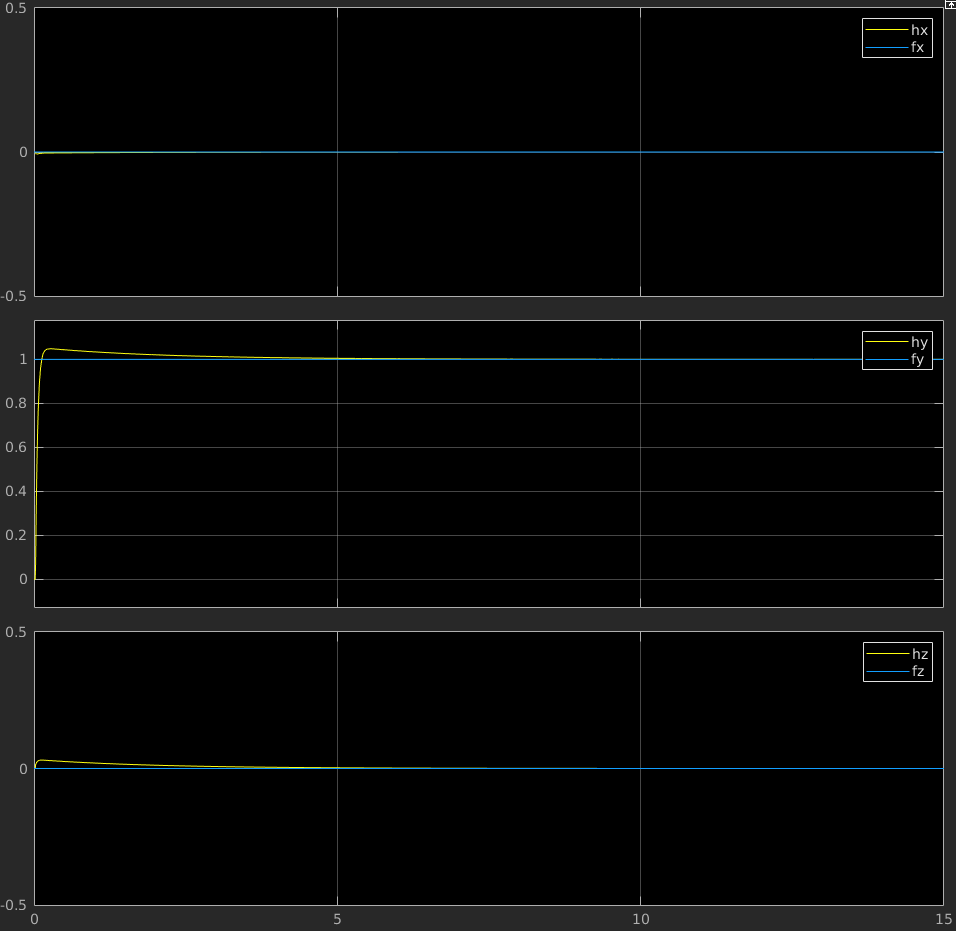
\includegraphics[keepaspectratio,width=0.6\textwidth]{force_1}
\caption{Force control with inner position loop - $C_F=K_F+\frac{1}{s}K_I$}
\end{figure}

\begin{figure}[h]
\centering
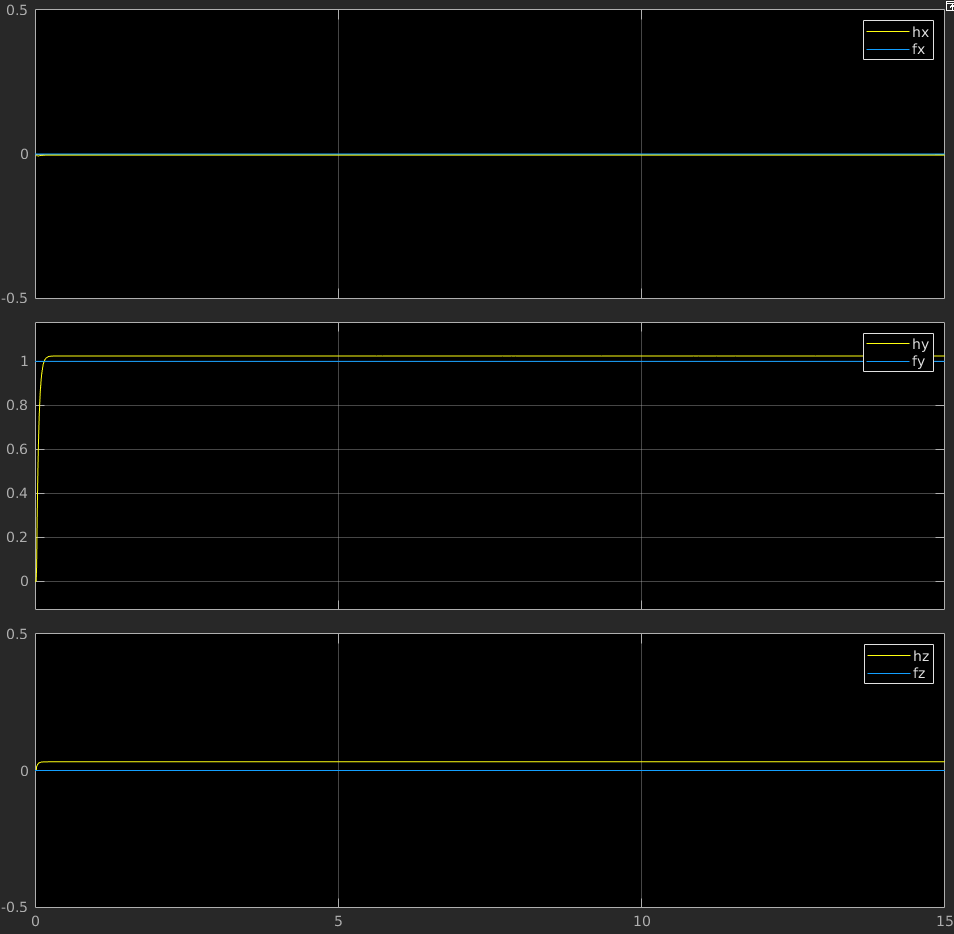
\includegraphics[keepaspectratio,width=0.6\textwidth]{force_noi}
\caption{Force control with inner position loop - $C_F=K_F$}
\end{figure}